%
% Chapter : Using the BLA in ILC for DPD
%
\section{Introduction}
\section{The Blocky Tought Experiment}

		A nonlinear dynamic system can alternatively be represented by the combination of a linear transfer function $G_{BLA}$ and a nonlinear function F.
		\begin{figure}[hbtp]
			\centering
			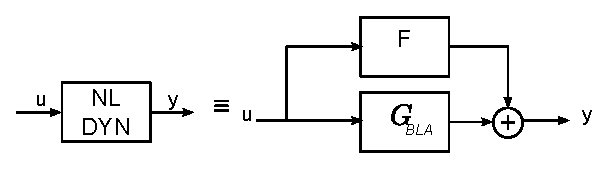
\includegraphics{images/lego1}
			\caption{Alternative representations of a nonlinear system. }
		\end{figure}
	
		\begin{figure}[hbtp]
			\centering
			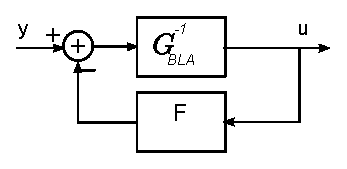
\includegraphics{images/lego2}
			\caption{Switching the input and output, creating the inverse of the nonlinear system. }
		\end{figure}

		\begin{figure}[hbtp]
			\centering
			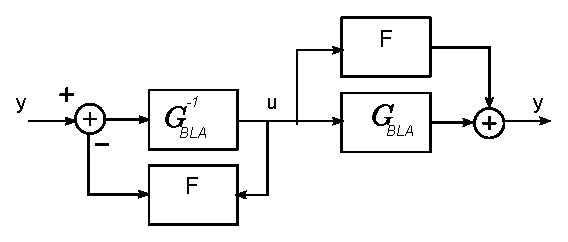
\includegraphics{images/lego3}
			\caption{Connecting the inverse and the original system together. }
		\end{figure}

		\begin{figure}[hbtp]
			\centering
			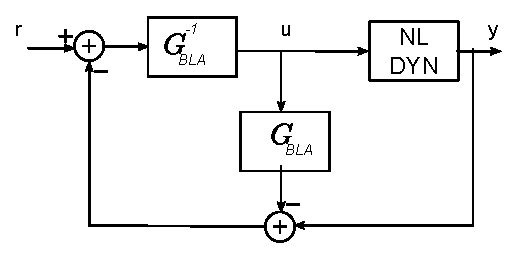
\includegraphics{images/lego4}
			\caption{Getting creative with the blocks. }
		\end{figure}

		\begin{figure}[hbtp]
			\centering
			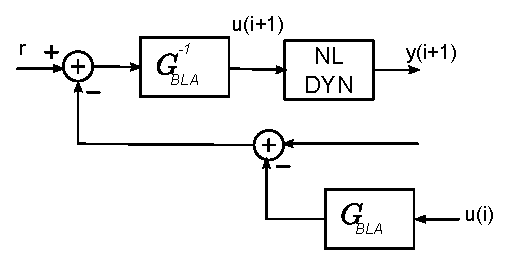
\includegraphics{images/lego5}
			\caption{Cut the loop! }
		\end{figure}

		\begin{figure}[hbtp]
			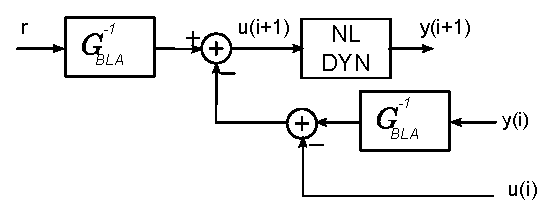
\includegraphics{images/lego6}
			\caption{Reorganise the blocks one last time. }
		\end{figure}

\section{Why can it work?}

\begin{enumerate}
	\item 
\end{enumerate}